\documentclass[10pt]{article}
 
\usepackage[margin=2cm]{geometry} 
\usepackage{amsmath,amsthm,amssymb, graphicx, multicol, array}
\usepackage[utf8]{inputenc}	% für Umlaute ect.
\usepackage{hyperref}
\usepackage{enumitem}
\usepackage{advdate}
\usepackage{esvect}
\usepackage{url}
\usepackage{hyperref}
\usepackage{listings}

\usepackage{color}
\definecolor{gray}{rgb}{0.4,0.4,0.4}
\definecolor{darkblue}{rgb}{0.0,0.0,0.6}
\definecolor{cyan}{rgb}{0.0,0.6,0.6}

\lstset{
	basicstyle=\ttfamily,
	columns=fullflexible,
	showstringspaces=false,
	commentstyle=\color{gray}\upshape
}

\lstdefinelanguage{XML}
{
	morestring=[b]",
	morestring=[s]{>}{<},
	morecomment=[s]{<?}{?>},
	stringstyle=\color{black},
	identifierstyle=\color{darkblue},
	keywordstyle=\color{cyan},
	morekeywords={xmlns,version,type}% list your attributes here
}
 
\DeclareMathOperator*{\argmax}{arg\,max}
\newcommand{\N}{\mathbb{N}}
\newcommand{\Z}{\mathbb{Z}}
 
%\newenvironment{problem}[2][Problem]{\begin{trivlist}
%\item[\hskip \labelsep {\bfseries #1}\hskip \labelsep {\bfseries #2.}]}{\end{trivlist}}

\newcounter{problemCounter}
\newenvironment{problem}[1]
{
	\vspace{0.5cm}
	\refstepcounter{problemCounter}\label{#1}
	\noindent \textbf{Problem \theproblemCounter.$\;$} 
}{}

\newcounter{solutionCounter}
\newenvironment{solution}[1] {%
	\vspace{0.5cm}
	\refstepcounter{solutionCounter}\label{#1}
	\noindent \textbf{Solution \theproblemCounter.}~% 
} {%
\vspace{0.5cm}
}

\begin{document}
 
\title{ Project - Latent Dirichlet Allocation \\
	Graphische Modelle (Lab)}
\author{Release: \today \; Submit: \AdvanceDate[32]\today.\\}
\date{}
\maketitle

In this project you will implement a document exploration system for the \href{https://simple.wikipedia.org/wiki/Main_Page}{Simple English Wikipedia}: Given an article, we want to obtain a number of similar articles, that can be used for recommendation and exploration. For this you will implement the Latent-Dirichlet-Allocation inference algorithm, based on on Gibbs sampling as described in \cite{heinrich:pefta}. Finally you will have to write a project report where you present your implementation and results. \\

Notes:
\begin{itemize}
	\item You can either chose Python or C++ as a programming language for your implementation.
	\item You are allowed and encouraged to work in teams.
	\item You must submit your code and your individually written project report. The oral exam will be based on your submissions.
	\item The baseline to pass the exam is a working implementation of the LDA inference algorithm.
	\item Start early with the implementation process!
	\item Ask, if there are problems.
\end{itemize}

\section{Latent Dirichlet Allocation}
\begin{problem}
	TThe LDA - Generative model \\
	Implement the LDA generative model as described in \cite{heinrich:pefta}. Thus, write a function that creates documents, given a number of topics.
\end{problem}

\begin{problem}
	IImplement the LDA inference algorithm, based on Gibbs sampling as described in \cite{heinrich:pefta}. Use your generative model to test the correctness of your implementation. First, focus on correctness but note that you will also need to optimize you code for performance for the later project.
\end{problem}

\section{Topic modeling with Wikipedia}

The \href{https://simple.wikipedia.org/wiki/Main_Page}{Simple English Wikipedia} is an edition of the English Wikipedia written in basic English. The articles on the Simple English Wikipedia are, in general, shorter, use a limited vocabulary and grammatically less complex. Currently (November 2018) it contains a set of 140.794 articles. You will need to obtain a copy of the whole archive, preprocess the document and learn a model upon it.

\begin{problem}
	DData gathering \\
	Get the latest XML dump of the Simple English Wikipedia from  \href{https://dumps.wikimedia.org/simplewiki/20181120/}{here}. We are interested in the "All pages, current versions only" which excludes media files. Once you have downloaded the archive ($\sim$ 200.0 MB), unpack the XML file ($\sim 1.2 GB$).
\end{problem} \\
The XML file is structured in the following way:
\begin{lstlisting}[language=XML]
<mediawiki>
  <siteinfo> ... </siteinfo>
  <page> page 1: content </page>
    ....
  <page> page M: content </page>
</mediawiki>
\end{lstlisting}
Each page corresponds to one Wikipedia article. E.g. the page for article "April" looks as follows:
\begin{lstlisting}[language=XML]
<page>
  <title>April</title>
  <ns>0</ns>
  <id>1</id>
  <revision>
    <id>6286716</id>
    <parentid>6213898</parentid>
    <timestamp>2018-10-24T19:26:39Z</timestamp>
    <contributor>
      <username>CommonsDelinker</username>
      <id>5295</id>
    </contributor>
    <comment>...</comment>
    <model>wikitext</model>
    <format>text/x-wiki</format>
    <text>
        HERE IS THE RELEVANT PART FOR US!
    </text>
    <sha1>h0cu2m6igv5zi77ekvich7a0byi1zuv</sha1>
  </revision>
<page>
\end{lstlisting}
For us there are two relevant tags:
\begin{enumerate}
  \item $<ns>$: The \href{https://en.wikipedia.org/wiki/Wikipedia:Namespace}{namespace} tag. We are only interested in articles in the namespace "$0$" which are the set of main articles.
  \item $<text>$: Contains the article content. Note here that for simplicity we only want to process the "introductory" text for each article (see fig. \ref{fig:article_intro}).
\end{enumerate}

\begin{figure}
	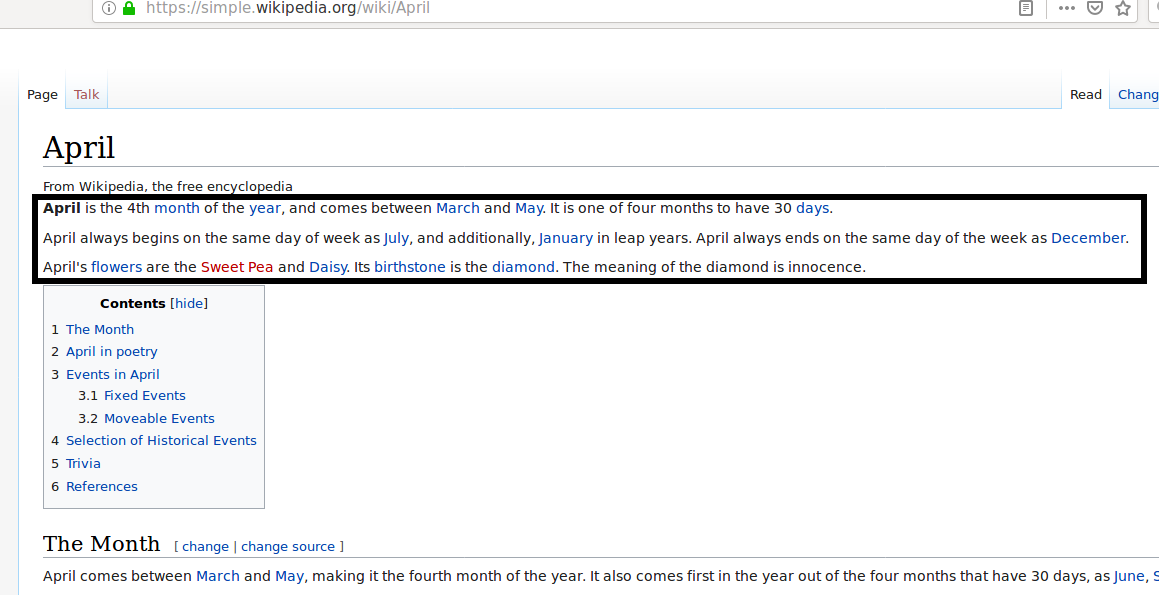
\includegraphics[width=0.9\textwidth]{article_intro.png}
	\label{fig:article_intro}
	\caption{The Simple English Wikipedia article for "April". We are interested in the introductory text (highlighted).}
\end{figure}

\begin{problem}
	PPreprocessing \\
	Extract the introductory text for each article. In Python you can use the \href{https://docs.python.org/3.7/library/xml.etree.elementtree.html}{XML} module to parse the document and extract the relevant text segments. Once obtained, you have to process the raw text segments that will make your documents:
	\begin{itemize}
		\item Tokenization: Split text documents into words, lowercase the words and remove punctuation.
		\item Lemmatization: Words in third person are changed to first person and verbs in past and future tenses are changed into present. Words are reduced to their root form.
		\item Remove stopwords, since they are not expressive in our model.
		\item Remove wikipedia specific expressions and tags. E.g "[[Some Text]]" should be transformed into "Some text". and "[[File:ColorfulSpringGarden.jpg|thumb|180px|right|[[Spring]]" should be transformed into "Spring".
		\item Remove numbers.
		\item ...
	\end{itemize}
	Your aim should be reduce the vocabulary size and ambiguity in your documents.
	You can also try to filter words that are rarely or frequently used. Most of the relevant functions are already implemented and you can make used of them. In Python you can checkout the 
	\href{https://radimrehurek.com/gensim/parsing/preprocessing.html}{gensim module}. It offers broad support for most preprocessing requirements.
\end{problem}

\begin{problem}
	TTraining the model \\
	Train a model with your implementation of the LDA inference algorithm. To start with, use a properly sized subset of your whole document corpus. Since the key problem with unsupervised learning techniques like LDA is the validation of your results you will need manual validation to make sense of the results. Additionally there are various result visualization tools like \href{https://github.com/bmabey/pyLDAvis}{pyLDAvis} that deliver great insights into your training results (see \ref{fig:pyldavis}).
\end{problem}

\begin{figure}
	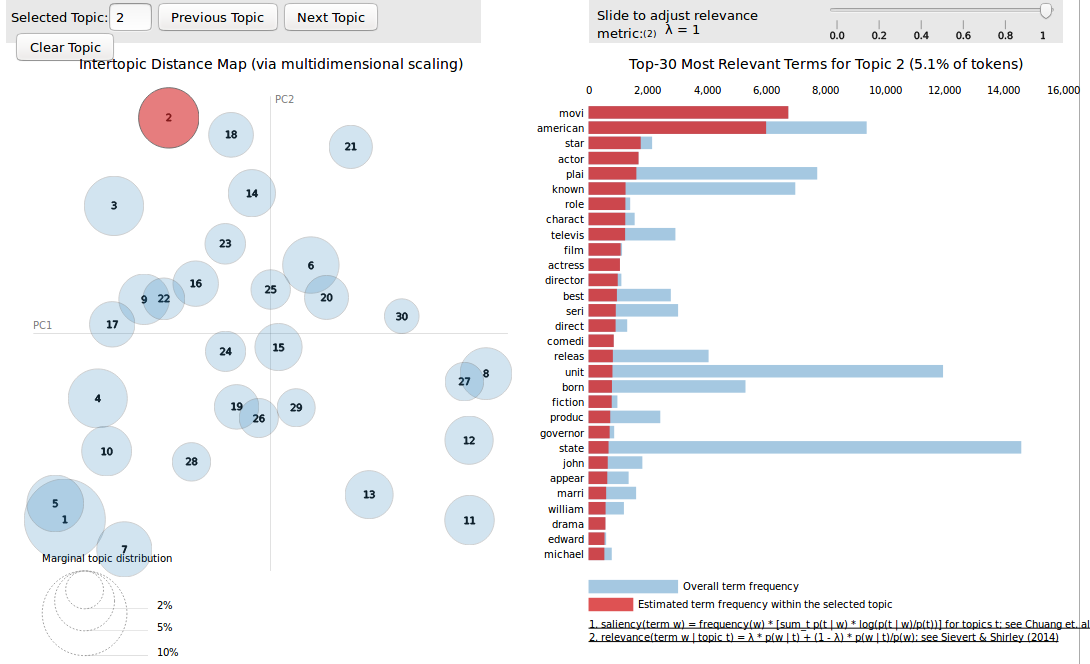
\includegraphics[width=0.9\textwidth]{pyldavis.png}
	\label{fig:pyldavis}
	\caption{pyLDAvis in action.}
\end{figure}

\begin{problem}
	DDocument exploration and recommendation \\
	Given your model we want to able to answer queries of the form: Given article $A$, what are the $k$ most similar articles $B_1, ...,B_k$. As an use case, you can think of article recommendation for users of the Wikipedia. \\
	For this task you need a similarity measure, based on the document-topic distribution to compare documents. One possible measure is the \href{https://en.wikipedia.org/wiki/Jensen%E2%80%93Shannon_divergence}{Jensen–Shannon divergence}.
	Once done, you can use this tool to ask and answer further questions ;)
\end{problem}

\section{Project report}

\begin{problem}
	WWrite a project report of approx. 5 - 10 content pages. Introduce the LDA model and write about your approach to solve the inference problems. Don't be overly verbose and stay formal whenever you can, but the report should be self-contained. Write about your implementation. Deliver performance results and give key insights. Write about your experiments on the Simple English Wikipedia dataset.
	Possible questions. Also reference ALL your resources.
\end{problem} \\

\begin{center}
	Happy Coding!
\end{center}
\newpage

\bibliography{references} 
\bibliographystyle{ieeetr}

\end{document}